\documentclass{article}
\usepackage[utf8]{inputenc}
\usepackage{tikz}
\usepackage{pgf}
\title{DAG_OSFP}
\author{francois.bettega+overleaf }
\date{January 2022}

\begin{document}



% This code uses the tikz package
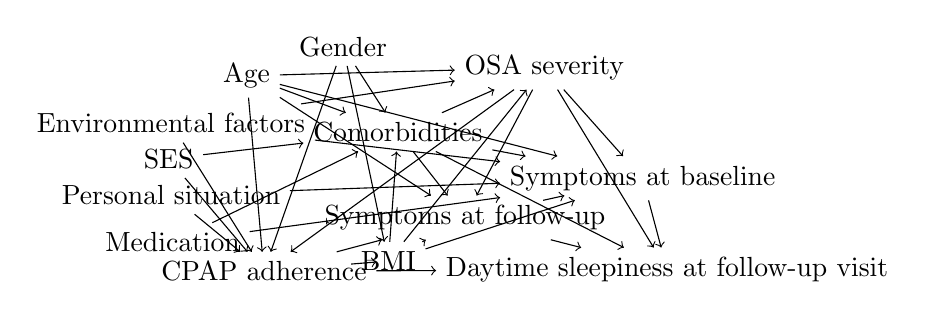
\begin{tikzpicture}
\node (v0) at (-1.95,-1.97) {CPAP adherence};
\node (v1) at (3.17,-1.95) {Daytime sleepiness at follow-up visit };
\node (v2) at (-3.13,-0.0910) {Environmental factors};
\node (v3) at (1.61,0.615) {OSA severity};
\node (v4) at (-3.13,-1.00) {Personal situation};
\node (v5) at (2.86,-0.789) {Symptoms at baseline};
\node (v6) at (0.603,-1.29) {Symptoms at follow-up};
\node (v7) at (-2.17,0.512) {Age};
\node (v8) at (-0.370,-1.84) {BMI};
\node (v9) at (-0.248,-0.203) {Comorbidities};
\node (v10) at (-0.945,0.884) {Gender};
\node (v11) at (-3.11,-1.60) {Medication};
\node (v12) at (-3.16,-0.541) {SES};
\draw [->] (v0) edge (v1);
\draw [->] (v0) edge (v6);
\draw [->] (v2) edge (v0);
\draw [->] (v2) edge (v3);
\draw [->] (v2) edge (v5);
\draw [->] (v3) edge (v0);
\draw [->] (v3) edge (v1);
\draw [->] (v3) edge (v5);
\draw [->] (v3) edge (v6);
\draw [->] (v4) edge (v0);
\draw [->] (v4) edge (v5);
\draw [->] (v5) edge (v1);
\draw [->] (v5) edge (v6);
\draw [->] (v6) edge (v1);
\draw [->] (v7) edge (v0);
\draw [->] (v7) edge (v3);
\draw [->] (v7) edge (v5);
\draw [->] (v7) edge (v6);
\draw [->] (v7) edge (v9);
\draw [->] (v8) edge (v0);
\draw [->] (v8) edge (v3);
\draw [->] (v8) edge (v5);
\draw [->] (v8) edge (v6);
\draw [->] (v8) edge (v9);
\draw [->] (v9) edge (v1);
\draw [->] (v9) edge (v3);
\draw [->] (v9) edge (v5);
\draw [->] (v9) edge (v6);
\draw [->] (v10) edge (v0);
\draw [->] (v10) edge (v8);
\draw [->] (v10) edge (v9);
\draw [->] (v11) edge (v5);
\draw [->] (v11) edge (v9);
\draw [->] (v12) edge (v0);
\draw [->] (v12) edge (v9);
\end{tikzpicture}





\end{document}
